\documentclass[11pt]{article} \usepackage[top=2cm, bottom=2cm, left=2cm, right=2cm]{geometry}
\usepackage[francais]{babel} \usepackage{fontspec} % remplace \usepackage[utf8]{inputenc} et \usepackage[T1]{fontenc}
\usepackage{amsmath} \usepackage{amsfonts} \usepackage{amssymb} \usepackage{algorithm} \usepackage{algpseudocode}
\usepackage[babel=true]{csquotes} % csquotes va utiliser la langue définie dans babel
\usepackage{xcolor}
% ------------Raccourcis-------------
\newcommand{\abs}[1]{\left\lvert#1\right\rvert} \newcommand{\norm}[1]{\left\lVert#1\right\rVert}
\newcommand{\pars}[1]{\left(#1\right)} \newcommand{\bigpars}[1]{\bigl(#1\bigr)} \newcommand{\set}[1]{\left\{#1\right\}}
\newcommand{\floor}[1]{\lfloor #1 \rfloor} \newcommand{\ceil}[1]{\lceil #1 \rceil}



\title{ACVL} \title{Le problème du voyageur de commerce} \author{SALL Amadou \and PIGN\'E Quentin } \date{\today}
\begin{document}

\maketitle
\section{Structure de données}
Nous avons dans un premier temps développé la structure de données servant à modéliser un graphe. Elle comporte une liste de sommets ainsi qu'une liste d'arcs, implémentées avec de simples \texttit{List} Java. Une telle structure est nécessaire pour afficher les graphes et vérifier leur complétude. Cependant afin de nous faciliter la tâche pour les algorithmes, nous avons décidé d'ajouter au graphe une matrice des distances entre sommets. La graphe étant complet et non orienté, la matrice est symétrique et chaque case représente un arc. Une telle structure nous permettra par exemple de facilement et rapidement récupérer toutes les distances des arcs partant d'un sommet. Ainsi, les algorithmes que nous avons implémenté n'utilisent que cette matrice des
distances qui à elle seule définie le graphe.
\section{Algorithmes}
Pour chaque figure, la courbe \textcolor{blue}{bleu} est celle obtenue avec nos valeurs expérimentales alors que la \textcolor{red}{rouge} est la complexité théorique.
\subsection*{Floyd-Warshall}
$d^{k+1}(i,j)$ est le plus court chemin de $i$ à $j$ n'utilisant que les sommets $\set{1,\cdots,k+1}$ comme sommet intermédiaires. Dès lors, il n'y a que deux cas possibles :
\begin{description}
    \item[on passe par le sommet $k+1$ :]  dans ce cas, il faut aller de $i$ à $k+1$ de façon optimale (coût $d^{k}(i,k+1)$) puis quitter $k+1$ pour aller jusqu'à $j$ de façon optimale aussi (coût $d^{k}(k+1,j)$)
\item[on ne passe pas par le sommet $k+1$ :] dans ce cas on a toujours un coût de $d^{k}(i,j)$
\end{description}
Ainsi on a la formule :
\begin{displaymath}
  d^{k+1}(i,j) = d^{k}(i,k+1) + d^{k}(k+1,j) 
\end{displaymath}
Le but étant calculer la matrice des $d^{n}(i,j)$, le coeur de l'algorithme de Floyd-Warshall s'écrit :
  \begin{algorithmic}[]
   \For{$k \gets 1,n$}
       \For{$i \gets 1,n$}
           \For{$ \gets 1,n$}
           \State $ d^{k+1}(i,j) = d^{k}(i,k+1) + d^{k}(k+1,j) $
           \EndFor
       \EndFor
   \EndFor
  \end{algorithmic}
Ainsi, l'algorithme de Floyd-Warshall a un coût de $O(n^3)$.

\subsection*{\'Enumération}
Cet algorithme a un coût en $O(n!)$. En effet lors à l'étape $k$ on a $k-1$ choix. Pour faire donc les $n$ étapes, on a un coût de $(n-1)!$. On a aussi $n$ possibilités pour le choix d'un noeud de départ.
  \begin{figure}[ht]
\begin{center}
  
  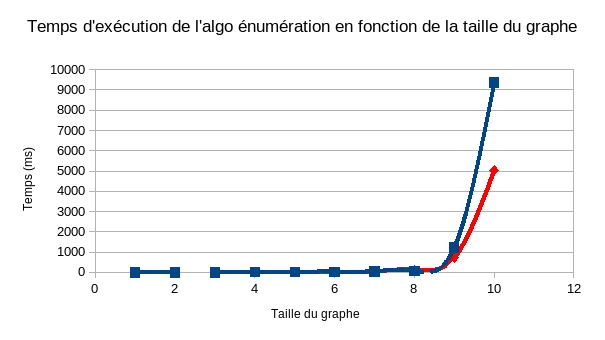
\includegraphics[scale=0.8]{images/exec_enum.png}
  \caption{Analyse de perfomances pour \'Enumération}
  \label{fig:enum}
\end{center}
\end{figure}
Après avoir tester l'algorithme sur des graphes de différentes taille, nous avons pu voir que la taille maximale est $n=10$. Ensuite, afin de tester le coût de l'algorithme en pratique, nous avons générer 10 graphes différents de tailles 1 à 10, puis nous avons mesurer le temps de calcul pour chaque graphe avant d'en tracer l'évolution. Ainsi, la figure \ref{fig:enum} montre que le temps d'exécution de l'algorithme d'énumération est bien en $O(n!)$.

\subsection*{Algorithme glouton}
Il y a $n$ possibilités pour le choix du sommets de départ. Une fois celui-ci choisi (que nous appellerons $i$), on choisit le sommet qui minimise la distance. À l'étape $k$, on doit choisir entre les $k-1$ sommets restants, soit $k-1$ valeurs possibles. Ce qui donne au final un coût de l'algorithme en $k-1$. Au total, on a $O(\sum_{k=1}^{n-1} k)$ opérations. 
Ainsi l'algorithme glouton a un coût en $O(n^2)$.
Le graphe ci-après présente l'étude numérique de la complexité de l'algorithme glouton, mesuré selon le même protocole expérimental que précédemment.
  \begin{figure}[ht]
\begin{center}
  
  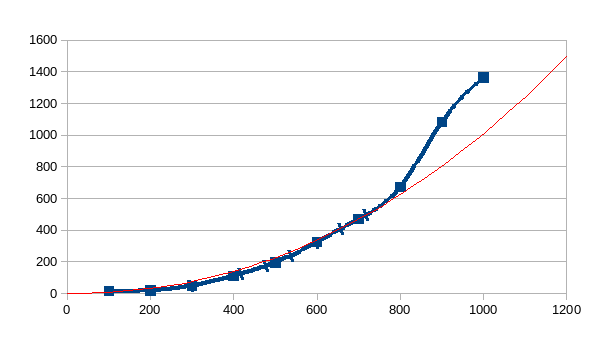
\includegraphics[scale=0.8]{images/exec_glouton.png}
  \caption{Analyse de perfomances pour L'algorithme glouton}
  \label{fig:glouton}
\end{center}
\end{figure}
On retrouve donc ainsi une complexité en $O(n^2)$.
\subsection*{Algorithme de recherche locale}
Pour un arc donné, disons $(u,v)$, le nombre d'arcs à tester est $n-4$. Et on a $n-1$ possibilités pour le choix de $(u,v)$. Le coût de la recherche locale est donc en $O(n^2)$. Bien que de même complexité que l'algorithme glouton, on peut se rendre compte en pratique que l'amélioration apportée par le recherche locale peut atteindre plus de 50\%. Cependant $O(n^2)$ est dans cette situation un coût moyen et la complexité au pire cas est exponentielle.
  \begin{figure}[ht]
\begin{center}
  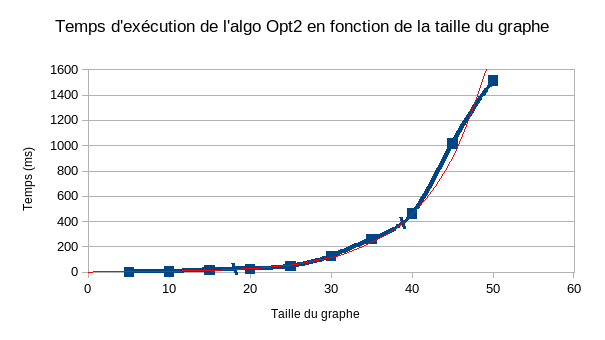
\includegraphics[scale=0.8]{images/exec_opt2.png}
  \caption{Analyse de perfomances pour 2-OPT}
  \label{fig:opt2}
\end{center}
\end{figure}
Lors de la mesure expérimentale de la complexité de l'algorithme, les résultats obtenus on mis en évidence un coût exponentiel (voir figure \ref{fig:opt2}). Cela est probablement dû au fait que nous testions l'algorithme sur une seule et même réalisation de l'algorithme glouton.
\subsection*{Programmation dynamique}
Dans le chemin correspondant à $C(S,j)$ le prédécesseur $i_0$ de $j$ est l'un des $|S|-1$ éléments de
$\set{S} \backslash \set{j}$. Il faut arriver jusqu'à $i_0$ en passant par le plus court chemin utilisant une et une
seule fois les sommets de $\set{S} \backslash \set{j}$. Ainsi le coût est 
$C(\set{S} \backslash \set{j},i_0) + l_{(i_0,j)}$. Le $i_0$ correspondant est celui qui minimise la précédente somme car
sinon on serait passé par autre \enquote{prédécesseur potentiel} de $j$. Ainsi on a :
\begin{displaymath}
  C(S,j) = min_{i \in S , i \neq j}C(\set{S} \backslash \set{j},i)) + l_{(i,j)}
\end{displaymath}
La solution au problème est $C(E,n)$.
 Le nombre de sous-ensembles de $\set{1,\cdots,n}$ est $2^n$. Chacun de ces sous-ensembles contient $O(n)$ sommets. Pour
 un sommet $j$ de $S$, le calcul de $C(S,j)$ nécessite $O(n)$ opérations. 

Ainsi la programmation dynamique a un coût en $O(n^22^n)$

l'algorithme de programmation dynamique peut s'écrire :
%\begin{algorithm}[!ht]
%\caption{Programmation dynamique pour le TSP}
\begin{algorithmic}[]
%\Require une matrice de poids, un ensemble de $n$ sommets
\For{chaque sous-ensemble $S$ commençant par $1$}
\If{$|S| = 2$}
\For{$i$ de $1$ à $n$}
\State $C(S,i) \gets l_{(1,i)}$
\EndFor
\Else
\For{$i$ de $1$ à $n$}
\For{tous les $k$ $\notin$ $S - \{ 1 \}$}
\State $C(S,i) \gets \min$ $\{$ $C(S - \{ k \} ,k)$ + $l_{(k,i)}$ $\}$
\EndFor
\EndFor
\EndIf
\EndFor
\State retourner $\min$ $\{$ C(S,i) + $l_{(1,i)}$ $\}$ avec $|S| = $
(nombre de sommets - 1)
\end{algorithmic}
% \end{algorithm}
Faute de temps, nous n'avons malheureusement pas pu implémenter cet algorithme afin de pouvoir en tester la complexité.
\section{Comparaison des algorithmes}
\begin{description}
    \item[Avantage de la programmation dynamique sur l'énumération :] les sous-chemins du circuit minimal sous aussi
  minimaux, on ne teste donc pas tous les circuits possibles. La complexité passe de $O(n!)$ à $O(n^22^n)$
  \item[Avantage de la combinaison glouton + recherche locale :] L'algorithme glouton permet de trouver des solutions en
des temps raisonnables. Cependant la valeur trouvée n'est pas forcément l'optimum. Appliquer L'algorithme de recherche
locale permet de gagner très nettement en précision (50\%)
\item[Glouton + recherche locale vs programmation dynamique :] La programmation dynamique est beaucoup plus précise mais
le coût en patît forcément. Juste le stockage de la matrice des stockage coute $O(n2^n)$

\end{description}

\end{document}